\documentclass[12pt]{article}
\usepackage[explicit]{titlesec}
\setlength{\parindent}{0pt}
\setlength{\parskip}{1em}
\usepackage{hyphenat}
\usepackage{ragged2e}
\RaggedRight

\usepackage{caption}

% These commands change the font. If you do not have Garamond on your computer, you will need to install it.
%\usepackage{garamondx}
\usepackage[T1]{fontenc}
\usepackage{amsmath, amsthm}
\usepackage{graphicx}

% These packages are used for drawing flow chart
\usepackage{tikz}
\usetikzlibrary{shapes,arrows}

% This adjusts the underline to be in keeping with word processors.
\usepackage{soul}
\setul{.6pt}{.4pt}


% The following sets margins to 1 in. on top and bottom and .75 in on left and right, and remove page numbers.
\usepackage{geometry}
\geometry{vmargin={0.5in, 0.5in}, hmargin={.5in, .5in}}
\usepackage{fancyhdr}
\pagestyle{fancy}
\renewcommand{\headrulewidth}{0.0pt}
\renewcommand{\footrulewidth}{0.0pt}

% These Commands create the label style for tables, figures and equations.
\usepackage[labelfont={footnotesize,bf} , textfont=footnotesize]{caption}
\captionsetup{labelformat=simple, labelsep=period}
\newcommand\num{\addtocounter{equation}{1}\tag{\theequation}}
\renewcommand{\theequation}{\arabic{equation}}
\makeatletter
\renewcommand\tagform@[1]{\maketag@@@ {\ignorespaces {\footnotesize{\textbf{Equation}}} #1.\unskip \@@italiccorr }}
\makeatother
\setlength{\intextsep}{10pt}
\setlength{\abovecaptionskip}{2pt}
\setlength{\belowcaptionskip}{-10pt}

% These commands set the paragraph and line spacing
\titleformat{\section}
{\normalfont}{\thesection}{2em}{\MakeUppercase{\textbf{#1}}}
\titlespacing\section{0pt}{0pt}{-12pt}
\titleformat{\subsection}
{\normalfont}{\thesubsection}{2em}{\textit{#1}}
\titlespacing\subsection{0pt}{0pt}{-12pt}
\renewcommand{\baselinestretch}{1.2}

% This designs the title display style for the maketitle command
\makeatletter
\newcommand\twenty{\@setfontsize\twenty{20pt}{6}}
\renewcommand{\maketitle}{
	\begin{center}
		\vspace{-.375in}
		\twenty\bfseries \@title
		\medskip
	\end{center}
}
\makeatother

\title{Neural Networks (NN)}

\begin{document}
	
	\maketitle
	\justify
	
	%%%%%%%% Non-linear Model %%%%%%%%
	\section*{Non-linear Model}
	Logistic regression is good if we have 2 features in our problem, for example:
	
	%%%%%%%% FIGURE 1 %%%%%%%%
	\begin{figure}[ht!]
		\centering
		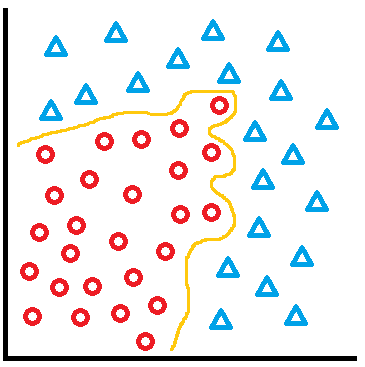
\includegraphics[scale=0.6]{figure1.png}
		\caption{Example of Logistic Regression Problem with 2 Features}
	\end{figure}
	%%%%%%%% FIGURE 1 %%%%%%%%
	
	However, if we have lots of features, we'll need to come up with hypothesis that include all of these features.
	
	With too many features, it might lead to overfitting problem and it can also be computationally expensive. Because of that, we'll need a new machine learning algorithm (Neural networks).
	
	%%%%%%%% Model Representation %%%%%%%%
	\section*{Model Representation}
	Neural networks was developed to simulate the networks of neurons in the brain. Some components in neural network include:
	\begin{itemize}
		\item Input wires
		\item Output wires
	\end{itemize}

	\underline{Neuron model: logistic unit:}
	
	%%%%%%%% FIGURE 2 %%%%%%%%%
	\begin{center}
		\tikzstyle{line} = [draw, -latex']
		\tikzstyle{vertex} = [draw, circle,fill=white!100, node distance=1.55em, minimum height=2em]
		\tikzstyle{inv_vertex} = [draw=none, circle,fill=white!100, node distance=1.5em, minimum height=0.5em]
		\tikzstyle{description} = [draw=none, rectangle,fill=white!100, node distance=2.1em, minimum height=1em]
		
		\begin{tikzpicture}[node distance = 2.1em, auto]
		% Place nodes
		\node [vertex] (x0) {$x_{0}$};
		\node [inv_vertex, below of=x0] (i0) {};
		\node [vertex, below of=i0] (x1) {$x_{1}$};
		\node [inv_vertex, below of=x1] (i1) {};
		\node [vertex, below of=i1] (x2) {$x_{2}$};
		\node [inv_vertex, below of=x2] (i2) {};
		\node [vertex, below of=i2] (x3) {$x_{3}$};
		\node [inv_vertex, below of=x3] (i3) {};
		\node [vertex, right of=i1, node distance=4em] (a0) {$a_{0}$};
		\node [description, right of=a0, node distance=8em] (h) {$h_\theta (x)=\frac{1}{1+e^{-\theta^{T}x}}$};
		\node [description, left of=x0, node distance=10em] (desc) {bias unit or bias neuron};
		
		% Draw edges
		\path [line] (x0) -- node {input wires} (a0);
		\path [line] (x1) -- (a0);
		\path [line] (x2) -- (a0);
		\path [line] (x3) -- (a0);
		\path [line] (a0) -- (h);
		\path [line] (desc) -- (x0);
		\end{tikzpicture}
		\captionof{figure}{An example of a neuron model}\label{labelname}
	\end{center}
	%%%%%%%% FIGURE 2 %%%%%%%%%
	
	The neuron in figure 2 is called an artificial neuron with a sigmoid activation function.
	
	\[\theta =
	\begin{bmatrix}
	\theta_{0} \\
	\theta_{1} \\
	\vdots \\
	\theta_{n}
	\end{bmatrix}
	\]
	
	The vector $\theta$ is called "parameters" or "weights"
	
	\underline{Neural network:}
	
	%%%%%%%% FIGURE 3 %%%%%%%%%
	\begin{center}
		\tikzstyle{line} = [draw, -latex']
		\tikzstyle{vertex} = [draw, circle,fill=white!100, node distance=1.55em, minimum height=2em]
		\tikzstyle{inv_vertex} = [draw=none, circle,fill=white!100, node distance=1.5em, minimum height=0.5em]
		\tikzstyle{description} = [draw=none, rectangle,fill=white!100, node distance=2.1em, minimum height=1em]
		
		\begin{tikzpicture}[node distance = 2.1em, auto]
		% Place nodes
		\node [inv_vertex] (i7) {};
		\node [vertex, below of=i7] (x0) {$x_{0}$};
		\node [inv_vertex, below of=x0] (i0) {};
		\node [vertex, below of=i0] (x1) {$x_{1}$};
		\node [inv_vertex, below of=x1] (i1) {};
		\node [vertex, below of=i1] (x2) {$x_{2}$};
		\node [inv_vertex, below of=x2] (i2) {};
		\node [vertex, below of=i2] (x3) {$x_{3}$};
		\node [inv_vertex, below of=x3] (i3) {};
		\node [vertex, right of=i7, node distance=6em] (a02) {$a_{0}^{(2)}$};
		\node [inv_vertex, below of=a02, node distance=2em] (i4) {};
		\node [vertex, below of=i4, node distance=3em] (a12) {$a_{1}^{(2)}$};
		\node [inv_vertex, below of=a12, node distance=2em] (i5) {};
		\node [vertex, below of=i5, node distance=3em] (a22) {$a_{2}^{(2)}$};
		\node [inv_vertex, below of=a22, node distance=2em] (i6) {};
		\node [vertex, below of=i6, node distance=3em] (a32) {$a_{3}^{(2)}$};
		\node [vertex, right of=i5, node distance=6em] (a13) {$a_{1}^{(3)}$};
		\node [description, right of=a13, node distance=6em] (h) {$h_{\Theta}(x)$};
		
		% Draw edges
		\path [line] (x0) -- (a12);
		\path [line] (x1) -- (a12);
		\path [line] (x2) -- (a12);
		\path [line] (x3) -- (a12);
		
		\path [line] (x0) -- (a22);
		\path [line] (x1) -- (a22);
		\path [line] (x2) -- (a22);
		\path [line] (x3) -- (a22);
		
		\path [line] (x0) -- (a32);
		\path [line] (x1) -- (a32);
		\path [line] (x2) -- (a32);
		\path [line] (x3) -- (a32);
		
		\path [line] (a02) -- (a13);
		\path [line] (a12) -- (a13);
		\path [line] (a22) -- (a13);
		\path [line] (a32) -- (a13);
		
		\path [line] (a13) -- (h);
		\end{tikzpicture}
		\captionof{figure}{An example of a neuron network}\label{labelname}
	\end{center}
	%%%%%%%% FIGURE 3 %%%%%%%%%
	
	Some new notations:
	\begin{itemize}
		\item $a_{i}^{(j)}$: "activation" of unit $i$ in layer $j$
		\item $\Theta^{(j)}$: matrix of \underline{weights} controlling function mapping from layer $j$ to layer $j+1$
	\end{itemize}

	For example:
	\begin{itemize}
		\item $\Theta^{(1)}$: the matrix of weights controlling function mapping from layer 0 to layer 1
		\item $\Theta_{12}^{(4)}$: the weight of the mapping from neuron 2 in layer 3 to neuron 1 in layer 4 
	\end{itemize}	

	Consider the example in figure 3, we will have:
	\begin{equation}
		a_1^{(2)} = g(\Theta_{10}^{(1)} x_0 + \Theta_{11}^{(1)} x_1 + \Theta_{12}^{(1)} x_2 + \Theta_{13}^{(1)} x_3)	
	\end{equation}
	\begin{equation}
		a_2^{(2)} = g(\Theta_{20}^{(1)} x_0 + \Theta_{21}^{(1)} x_1 + \Theta_{22}^{(1)} x_2 + \Theta_{23}^{(1)} x_3)
	\end{equation}
	\begin{equation}
		a_3^{(2)} = g(\Theta_{30}^{(1)} x_0 + \Theta_{31}^{(1)} x_1 + \Theta_{32}^{(1)} x_2 + \Theta_{33}^{(1)} x_3)
	\end{equation}
	\begin{equation}
		h_\Theta (x) = a_1^{(3)}  = g(\Theta_{10}^{(2)} a_0^{(2)} + \Theta_{11}^{(2)} a_1^{(2)} + \Theta_{12}^{(2)} a_2^{(2)} + \Theta_{13}^{(2)} a_3^{(2)})
	\end{equation}
	
	Consequently, we can see the matrix of the weights $\Theta$ as a 3-D matrix (sort of) as depicted in figure 4 below.
	
	%%%%%%%% FIGURE 4 %%%%%%%%%
	\begin{center}
		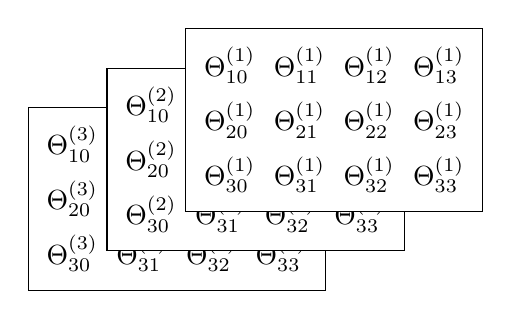
\begin{tikzpicture}
		\def\xs{1} %shift in x direction
		\def\ys{0.5} %shift in y direction
		\def\nm{1} % number of 2d matrices in the 3d matrix
		\foreach \x in {3,2,...,\nm}
		{
			
			\matrix [draw, % for the rectangle border
			fill=white, % so that it is not transparent
			ampersand replacement=\&] %see explanation
			(mm\x)%give the matrix a name
			at(-\x * \xs, -\x * \ys) %shift the matrix
			{
				\node {$\Theta_{10}^{(\x)}$}; \& \node {$\Theta_{11}^{(\x)}$}; \& \node {$\Theta_{12}^{(\x)}$}; \& \node {$\Theta_{13}^{(\x)}$}; \\
				\node {$\Theta_{20}^{(\x)}$}; \& \node {$\Theta_{21}^{(\x)}$}; \& \node {$\Theta_{22}^{(\x)}$}; \& \node {$\Theta_{23}^{(\x)}$}; \\
				\node {$\Theta_{30}^{(\x)}$}; \& \node {$\Theta_{31}^{(\x)}$}; \& \node {$\Theta_{32}^{(\x)}$}; \& \node {$\Theta_{33}^{(\x)}$}; \\
			};
		}
		
		\draw [dashed,gray](mm1.north west) -- (mm\nm.north west);
		\draw [dashed,gray](mm1.north east) -- (mm\nm.north east);
		\draw [dashed,gray](mm1.south east) -- (mm\nm.south east);
		\end{tikzpicture}
		\captionof{figure}{Visualization of matrix $\Theta$ for example in figure 3}\label{labelname}
	\end{center}
	%%%%%%%% FIGURE 4 %%%%%%%%%
	
	Consider an example of a neural network with 1 hidden layer having artificial neurons with a sigmoid activation function, we can write the activation functions in the hidden layer as follows:
	
	%%%%%%%% NEURAL NETWORK EXAMPLE %%%%%%%%
	\begin{center}
		\def\layersep{2.5cm}
		\begin{tikzpicture}[shorten >=1pt,->,draw=black!50, node distance=\layersep]
		\tikzstyle{every pin edge}=[<-,shorten <=1pt]
		\tikzstyle{neuron}=[draw, circle,fill=white!100,minimum size=25pt,inner sep=2pt]
		\tikzstyle{input neuron}=[neuron];
		\tikzstyle{output neuron}=[neuron];
		\tikzstyle{hidden neuron}=[neuron];
		\tikzstyle{annot} = [text width=4em, text centered]
		
		% Draw the input layer nodes
		\foreach \name/\y in {0,...,3}
		% This is the same as writing \foreach \name / \y in {1/1,2/2,3/3,4/4}
		\node[input neuron, pin=left:Input \#\y] (I-\name) at (0,-\y) {$a_{\y}^{(1)}$};
		
		% Draw the hidden layer nodes
		\foreach \name/\y in {0,...,3}
		\path[yshift=0.0cm]
		node[hidden neuron] (H-\name) at (\layersep,-\y cm) {$a_{\y}^{(2)}$};
				
		% Draw the output layer node
		\node[output neuron,pin={[pin edge={->}]right:Output}, right of=H-2] (O) {$a_1^{(3)}$};
		
		% Connect every node in the input layer with every node in the (except the bias node)
		% hidden layer.
		\foreach \source in {0,...,3}
		\foreach \dest in {1,...,3}
		\path (I-\source) edge (H-\dest);
		
		% Connect every node in the hidden layer with the output layer
		\foreach \source in {0,...,3}
		\path (H-\source) edge (O);
		
		% Annotate the layers
		\node[annot,above of=H-1, node distance=2.3cm] (hl) {Hidden layer};
		\node[annot,left of=hl] {Input layer};
		\node[annot,right of=hl] {Output layer};
		\end{tikzpicture}
	\end{center}
	%%%%%%%% NEURAL NETWORK EXAMPLE %%%%%%%%
	
	\begin{equation}
	a_1^{(2)} = g(\Theta_{10}^{(1)} a_0^{(1)} + \Theta_{11}^{(1)} a_1^{(1)} + \Theta_{12}^{(1)} a_2^{(1)} + \Theta_{13}^{(1)} a_3^{(1)}) = g(z_1^{(2)})
	\end{equation}
	\begin{equation}
	a_2^{(2)} = g(\Theta_{20}^{(1)} a_0^{(1)} + \Theta_{21}^{(1)} a_1^{(1)} + \Theta_{22}^{(1)} a_2^{(1)} + \Theta_{23}^{(1)} a_3^{(1)}) = g(z_2^{(2)})
	\end{equation}
	\begin{equation}
	a_3^{(2)} = g(\Theta_{30}^{(1)} a_0^{(1)} + \Theta_{31}^{(1)} a_1^{(1)} + \Theta_{32}^{(1)} a_2^{(1)} + \Theta_{33}^{(1)} a_3^{(1)}) = g(z_3^{(2)})
	\end{equation}
	\begin{equation}
	h_\Theta (x) = a_1^{(3)}  = g(\Theta_{10}^{(2)} a_0^{(2)} + \Theta_{11}^{(2)} a_1^{(2)} + \Theta_{12}^{(2)} a_2^{(2)} + \Theta_{13}^{(2)} a_3^{(2)}) = g(z^{(3)})
	\end{equation}
	
	When we consider $a_1^{(2)}$, $a_2^{(2)}$, $a_3^{(2)}$ as a whole, we can see the vectorized computation of the layer 2 (hidden layer) of the neural network as $\Theta^{(1)} a^{(1)}$ with $\Theta^{(1)}=\begin{pmatrix} \Theta_{10}^{(1)} & \Theta_{11}^{(1)} & \Theta_{12}^{(1)} & \Theta_{13}^{(1)} \\ \Theta_{20}^{(1)} & \Theta_{21}^{(1)} & \Theta_{22}^{(1)} & \Theta_{23}^{(1)} \\ \Theta_{30}^{(1)} & \Theta_{31}^{(1)} & \Theta_{32}^{(1)} & \Theta_{33}^{(1)} \\ \end{pmatrix}$ and $a^{(1)}=\begin{pmatrix} a_0^{(1)} \\ a_1^{(1)} \\ a_2^{(1)} \\ a_3^{(1)} \\ \end{pmatrix}$
	
	Consider $a^{(1)}=\begin{pmatrix} a_0^{(1)} \\ a_1^{(1)} \\ a_2^{(1)} \\ a_3^{(1)} \\ \end{pmatrix}$ and $z^{(2)}=\begin{pmatrix} z_1^{(2)} \\ z_2^{(2)} \\ z_3^{(2)} \\ \end{pmatrix}$, we'll have $z^{(2)}=\Theta^{(1)} a^{(1)}$. Therefore, the activation functions of layer 2 would be $a^{(2)}=g(z^{(2)})$
	
	After that, since we define the bias neuron in each layer as 1 by default, we'll add $a_0^{(2)}=1$ into the newly computed vector $a^{(2)}$.
	
	Finally, the hypothesis would be the activation function(s) of the output layer, which can be computed as follows: $z^{(3)}=\Theta^{(2)} a^{(2)}$ and $h_\Theta (x)=a^{(3)}=g(z^{(3)})$
	
	This process of computing $h_\Theta (x)$ is called \underline{forward propagation}: we start with the activations of the input units and forward propagate that to the hidden layers and compute the activations of the hidden layers and then forward propagate to compute activation(s) of the output layer. 
	
	Some other neural network architectures:
	
	%%%%%%%% NEURAL NETWORK EXAMPLE %%%%%%%%
	\begin{center}
		\def\layersep{2.5cm}
		\begin{tikzpicture}[shorten >=1pt,->,draw=black!50, node distance=\layersep]
		\tikzstyle{every pin edge}=[<-,shorten <=1pt]
		\tikzstyle{neuron}=[draw, circle,fill=white!100,minimum size=25pt,inner sep=2pt]
		\tikzstyle{input neuron}=[neuron];
		\tikzstyle{output neuron}=[neuron];
		\tikzstyle{hidden neuron}=[neuron];
		\tikzstyle{annot} = [text width=4em, text centered]
		
		% Draw the input layer nodes
		\foreach \name/\y in {0,...,3}
		% This is the same as writing \foreach \name / \y in {1/1,2/2,3/3,4/4}
		\node[input neuron] (I-\name) at (0,-\y) {};
		
		% Draw the hidden layer nodes
		\foreach \name/\y in {0,...,4}
		\path[yshift=0.5cm]
		node[hidden neuron] (H-\name) at (\layersep,-\y cm) {};
		
		% Draw the output layer node
		\node[output neuron, right of=H-2] (O) {};
		
		% Connect every node in the input layer with every node in the (except the bias node)
		% hidden layer.
		\foreach \source in {0,...,3}
		\foreach \dest in {0,...,4}
		\path (I-\source) edge (H-\dest);
		
		% Connect every node in the hidden layer with the output layer
		\foreach \source in {0,...,4}
		\path (H-\source) edge (O);
		
		\end{tikzpicture}
	\end{center}
	%%%%%%%% NEURAL NETWORK EXAMPLE %%%%%%%%
	
	%%%%%%%% NEURAL NETWORK EXAMPLE %%%%%%%%
	\begin{center}
		\def\layersep{5cm}
		\begin{tikzpicture}[shorten >=1pt,->,draw=black!50, node distance=\layersep]
		\tikzstyle{every pin edge}=[<-,shorten <=1pt]
		\tikzstyle{neuron}=[draw, circle,fill=white!100,minimum size=25pt,inner sep=2pt]
		\tikzstyle{input neuron}=[neuron];
		\tikzstyle{output neuron}=[neuron];
		\tikzstyle{hidden neuron}=[neuron];
		\tikzstyle{annot} = [text width=4em, text centered]
		
		% Draw the input layer nodes
		\foreach \name/\y in {0,...,7}
		% This is the same as writing \foreach \name / \y in {1/1,2/2,3/3,4/4}
		\node[input neuron] (I-\name) at (0,-\y) {};
		
		% Draw the hidden layer 1 nodes
		\foreach \name/\y in {0,...,4}
		\path[yshift=-1.5cm]
		node[hidden neuron] (H-\name) at (\layersep,-\y cm) {};
		
		% Draw the hidden layer 2 nodes
		\foreach \name/\y in {0,...,2}
		\path[yshift=-2.5cm]
		node[hidden neuron, right of=H-\name] (H1-\name) at (\layersep,-\y cm) {};
		
		% Draw the output layer nodes
		node[output neuron, right of=H1-2] (O) {};
		
		% Connect every node in the input layer with every node in the
		% hidden layer 1.
		\foreach \source in {0,...,7}
		\foreach \dest in {0,...,4}
		\path (I-\source) edge (H-\dest);
		
		% Connect every node in the input layer with every node in the
		% hidden layer 2.
		\foreach \source in {0,...,4}
		\foreach \dest in {0,...,2}
		\path (H-\source) edge (H1-\dest);
		
		% Connect every node in the hidden layer with the output layer
		\foreach \source in {0,...,2}
		\path (H1-\source) edge (O);
		
		\end{tikzpicture}
	\end{center}
	%%%%%%%% NEURAL NETWORK EXAMPLE %%%%%%%%
	
	%%%%%%%% NEURAL NETWORK EXAMPLE %%%%%%%%
	\begin{center}
		\def\layersep{5cm}
		\begin{tikzpicture}[shorten >=1pt,->,draw=black!50, node distance=\layersep]
		\tikzstyle{every pin edge}=[<-,shorten <=1pt]
		\tikzstyle{neuron}=[draw, circle,fill=white!100,minimum size=25pt,inner sep=2pt]
		\tikzstyle{input neuron}=[neuron];
		\tikzstyle{output neuron}=[neuron];
		\tikzstyle{hidden neuron}=[neuron];
		\tikzstyle{annot} = [text width=4em, text centered]
		
		% Draw the input layer nodes
		\foreach \name/\y in {0,...,12}
		% This is the same as writing \foreach \name / \y in {1/1,2/2,3/3,4/4}
		\node[input neuron] (I-\name) at (0,-\y) {};
		
		% Draw the hidden layer 1 nodes
		\foreach \name/\y in {0,...,7}
		\path[yshift=-2.5cm]
		node[hidden neuron] (H-\name) at (\layersep,-\y cm) {};

		% Draw the hidden layer 2 nodes
		\foreach \name/\y in {0,...,5}
		\path[yshift=-3.5cm]
		node[hidden neuron, right of=H-\name] (H1-\name) at (\layersep,-\y cm) {};
		
		% Draw the output layer nodes
		\foreach \name/\y in {1,...,4}
		\path[yshift=-4cm]
		node[output neuron, right of=H1-\name] (O-\name) {};
		
		% Connect every node in the input layer with every node in the
		% hidden layer 1.
		\foreach \source in {0,...,12}
		\foreach \dest in {0,...,7}
		\path (I-\source) edge (H-\dest);

		% Connect every node in the input layer with every node in the
		% hidden layer 2.
		\foreach \source in {0,...,7}
		\foreach \dest in {0,...,5}
		\path (H-\source) edge (H1-\dest);
		
		% Connect every node in the hidden layer with the output layer
		\foreach \source in {0,...,5}
		\foreach \dest in {1,...,4}
		\path (H1-\source) edge (O-\dest);
		
		\end{tikzpicture}
	\end{center}
	%%%%%%%% NEURAL NETWORK EXAMPLE %%%%%%%%
	
\end{document}